\documentclass[10pt,a4paper,twocolumn]{article}
\usepackage[utf8]{inputenc}
\usepackage[T1]{fontenc}
\usepackage[french]{babel}
\usepackage[margin=2cm]{geometry}
\usepackage{graphicx,booktabs,amsmath,hyperref,caption}
\graphicspath{{figures/}{../results/figures/}}

\title{Étude progressive des réseaux de neurones multicouches\\pour la reconnaissance d'activités humaines (HAR)}
\author{Alioune DIOP \and Madjiguène FALL\\M2 MALIA --- Deep Learning, 2026--2027}
\date{}

\begin{document}
\maketitle

% 6 pages maximum. Responsable de chaque section indiqué en commentaire.

\begin{abstract}
% Ensemble — à écrire en dernier.
\end{abstract}

\section{Introduction}               % Alioune
% Motivation, problématique, choix méthodologiques (validation par volontaire, graines, test unique).

\section{Données et prétraitements}  % Alioune
\subsection{Jeu de données HAR}
\subsection{Découpage apprentissage / validation}
% Tableau : validation par lignes vs par volontaire vs test.
\subsection{Référence : régression logistique}

%% ====================================================================== Madjiguène
\section{Architectures}              % Madjiguène
Tous les modèles sont des perceptrons multicouches de la forme
$[\mathrm{Linear}\to(\mathrm{BatchNorm})\to\mathrm{activation}\to(\mathrm{Dropout})]^{n}\to\mathrm{Linear}$,
avec 561 entrées (standardisées avec la moyenne et l'écart-type de l'apprentissage uniquement), 6 sorties
(logits) et la perte d'entropie croisée. L'entraînement utilise Adam, des lots de 64 exemples et trois
graines (0, 1, 2) ; les scores sont donnés en moyenne $\pm$ écart-type. Le tableau~\ref{tab:arch}
résume les architectures étudiées avec leur nombre de paramètres (la régression logistique de référence
en compte 3\,372). La version~1 correspond à la ligne $[64]$. Pour la version~2, nous retenons
$[256,128,64]$ avec les activations ReLU, ReLU, tanh : 185\,414 paramètres (186\,310 avec BatchNorm).

\begin{table}[t]
\centering\footnotesize
\setlength{\tabcolsep}{2pt}
\caption{Architectures et validation (Adam, 30 époques, 3 graines ; pour chaque architecture, meilleur
pas d'apprentissage et meilleure activation ; R = ReLU, T = tanh). $\Delta$ : accuracy
d'apprentissage moins accuracy de validation.}
\label{tab:arch}
\begin{tabular}{@{}lrccr@{}}
\toprule
Architecture & Params & F1 macro (val.) & $\Delta$ & Temps (s) \\
\midrule
\multicolumn{5}{@{}l}{\emph{Largeur (ReLU)}} \\
$[64]$ & 36\,358 & $0{,}9507\pm0{,}0026$ & 0,035 & 6,1 \\
$[128]$ & 72\,710 & $0{,}9500\pm0{,}0011$ & 0,041 & 6,7 \\
$[256]$ & 145\,414 & $0{,}9493\pm0{,}0043$ & 0,052 & 7,3 \\
\midrule
\multicolumn{5}{@{}l}{\emph{Profondeur (meilleure activation)}} \\
$[128,64]$, T & 80\,582 & $0{,}9447\pm0{,}0045$ & 0,060 & 6,9 \\
$[256,128,64]$, R-R-T & 185\,414 & $0{,}9418\pm0{,}0041$ & 0,064 & 9,1 \\
$[256,128,64,32]$, T & 187\,302 & $0{,}9367\pm0{,}0090$ & 0,066 & 9,3 \\
\bottomrule
\end{tabular}
\end{table}

\section{Résultats}
\subsection{MLP à une couche cachée}  % Alioune — activations, optimiseurs, LR, variabilité

\subsection{Largeur et profondeur}    % Madjiguène
Le pas d'apprentissage est choisi sur la validation parmi $\{10^{-4},3\!\cdot\!10^{-4},10^{-3},3\!\cdot\!10^{-3}\}$
pour la largeur (les trois premières valeurs pour la profondeur), avec un budget fixe de 30 époques et sans
arrêt anticipé, afin de comparer les architectures dans les mêmes conditions (tableau~\ref{tab:arch}).

\paragraph{Largeur.} Passer de 64 à 256 neurones multiplie les paramètres par quatre sans changer
le F1 de validation de façon détectable : l'écart maximal (0,0014) est inférieur aux écarts-types entre graines
(0,001 à 0,004). En revanche, l'écart entre accuracy d'apprentissage et de validation passe de 0,035 à 0,052 :
un réseau plus large sur-apprend davantage sans mieux généraliser. Le meilleur pas est le plus petit de la grille
pour les largeurs 64 et 128 ; avec 30 époques, un petit pas joue en partie le rôle d'un arrêt anticipé, donc
cette conclusion dépend du budget d'époques.

\paragraph{Profondeur et activations.} Ajouter des couches n'améliore pas la validation : le meilleur F1
passe de 0,945 (2 couches) à 0,942 (3) puis 0,937 (4), avec un écart d'apprentissage et un temps croissants
(6,9 à 9,3\,s). À profondeur donnée, les quatre combinaisons d'activations (ReLU, tanh, sigmoïde, ReLU puis
tanh) diffèrent de moins de 0,007 en F1 pour 2 et 3 couches, du même ordre que les écarts-types (0,004 à 0,012) :
on ne peut pas les départager. Le seul effet net est celui de 4 couches avec sigmoïde, qui n'apprend pas
(F1 $\approx 0{,}18$, accuracy $\approx 0{,}36$, quel que soit le pas testé), vraisemblablement à cause de
l'atténuation des gradients à travers des sigmoïdes empilées (explication non vérifiée).

\subsection{Régularisation}           % Madjiguène
Sur le réseau $[256,128,64]$ (ReLU, ReLU, tanh ; pas $3\!\cdot\!10^{-4}$, 30 époques), chaque technique est testée
isolément puis combinée (tableau~\ref{tab:reg}). Aucune technique seule n'améliore le F1 de façon détectable :
hors arrêt anticipé, les valeurs (0,930 à 0,938) sont dans la variabilité de la base (0,9418 $\pm$ 0,0041). L'arrêt
anticipé (patience 5) donne 0,9462, mais ce score est celui de la meilleure époque choisie sur la validation, donc
légèrement optimiste. En revanche, dropout 0,5, BatchNorm et arrêt anticipé réduisent la loss de validation
(0,30 $\to$ 0,23--0,25) : le réseau est moins sûr de lui à accuracy quasi constante. La combinaison BatchNorm
+ dropout 0,3 + weight decay + arrêt anticipé est la meilleure : F1 $0{,}9516\pm0{,}0052$, loss 0,159 et écart
d'apprentissage 0,027 contre 0,064. Ses variantes sans arrêt anticipé restent au niveau de la base (0,938 et 0,937),
ce qui suggère que l'arrêt anticipé en est l'ingrédient principal (hypothèse non isolée par nos essais).

La figure~\ref{fig:valloss} montre que la loss de validation remonte après quelques époques sans régularisation
forte, alors que le F1 reste stable. Aucune technique ne réduit l'instabilité du F1 d'une époque à l'autre
(écart-type entre époques : 0,006 pour la base, 0,0095 pour la combinaison, mesuré sur des runs de longueur
différente). Enfin, une recherche aléatoire de 30 configurations (bonus) ne trouve rien de significativement
meilleur : les trois meilleures, ré-évaluées sur 3 graines, atteignent 0,950 à 0,954, et le meilleur score à une
graine (0,957) retombe à 0,954, effet attendu de la sélection sur 30 essais.

\begin{table}[t]
\centering\footnotesize
\setlength{\tabcolsep}{2pt}
\caption{Régularisation de $[256,128,64]$ (validation, 3 graines). Dropout 0,1 et 0,3 : F1 0,9353 et 0,9358
(non montrés). AA : arrêt anticipé ; la loss et $\Delta$ sont pris à la meilleure époque pour les lignes avec AA.}
\label{tab:reg}
\begin{tabular}{@{}lccc@{}}
\toprule
Configuration & F1 macro & Loss val. & $\Delta$ \\
\midrule
Base (aucune) & $0{,}9418\pm0{,}0041$ & 0,300 & 0,064 \\
Dropout 0,5 & $0{,}9379\pm0{,}0038$ & 0,246 & 0,056 \\
Weight decay $10^{-4}$ & $0{,}9382\pm0{,}0058$ & 0,301 & 0,067 \\
BatchNorm & $0{,}9350\pm0{,}0034$ & 0,248 & 0,066 \\
AA (patience 5) & $0{,}9462\pm0{,}0050$ & 0,232 & 0,052 \\
BN + dropout 0,3 + wd + AA & $0{,}9516\pm0{,}0052$ & 0,159 & 0,027 \\
\bottomrule
\end{tabular}
\end{table}

\begin{figure}[t]
\centering
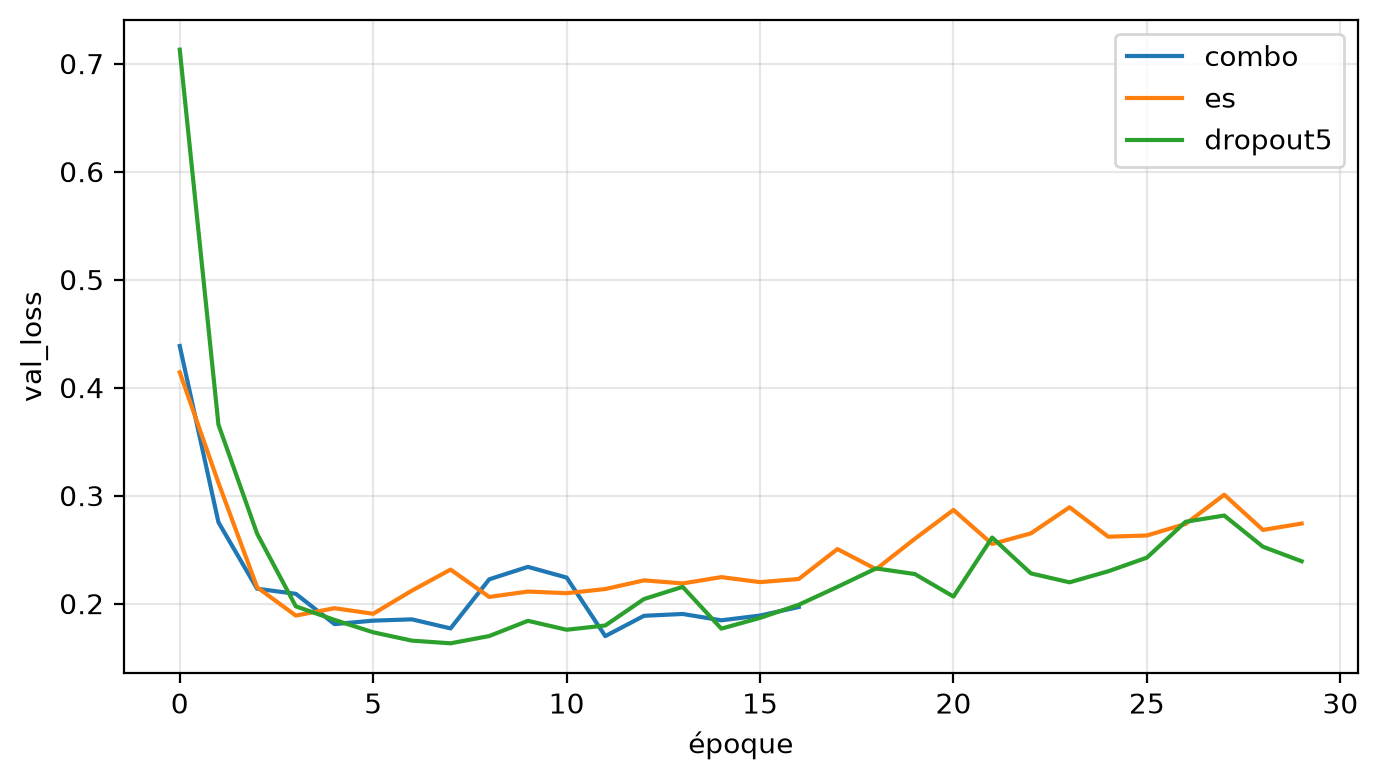
\includegraphics[width=\columnwidth]{v2_compare_loss}
\caption{Loss de validation (graine 0) des trois configurations retenues : \texttt{combo}, \texttt{es}
(arrêt anticipé seul) et \texttt{dropout5} (dropout 0,5).}
\label{fig:valloss}
\end{figure}

\subsection{Évaluation finale sur le test} % Alioune (référence + V1) · Madjiguène (V2) — tableau commun
Les trois configurations retenues sur la validation (\texttt{combo} : BatchNorm + dropout 0,3 + weight decay
+ arrêt anticipé ; \texttt{es} : arrêt anticipé seul ; \texttt{dropout5} : dropout 0,5) sont évaluées une seule fois
sur le test (2\,947 fenêtres, 9 volontaires absents de l'apprentissage et de la validation), avec 3 graines
(tableau~\ref{tab:test}).
% Alioune : ajouter au tableau commun les lignes « régression logistique » et « V1 [64] ».

\begin{table}[t]
\centering\footnotesize
\setlength{\tabcolsep}{2pt}
\caption{Évaluation finale de la version~2 : F1 macro en validation et au test (3 graines).
$\Delta$ : test moins validation.}
\label{tab:test}
\begin{tabular}{@{}lccc@{}}
\toprule
Configuration & F1 val. & F1 test & $\Delta$ \\
\midrule
\texttt{combo} & $0{,}9516\pm0{,}0052$ & $0{,}9369\pm0{,}0017$ & $-0{,}015$ \\
\texttt{es} & $0{,}9462\pm0{,}0050$ & $0{,}9262\pm0{,}0021$ & $-0{,}020$ \\
\texttt{dropout5} & $0{,}9379\pm0{,}0038$ & $0{,}9260\pm0{,}0073$ & $-0{,}012$ \\
% Alioune : lignes référence et V1
\bottomrule
\end{tabular}
\end{table}

Les trois configurations perdent entre 0,012 et 0,020 de F1 par rapport à la validation : celle-ci est
optimiste. \texttt{combo} reste la meilleure (F1 0,9369 $\pm$ 0,0017, accuracy 0,936). Son écart avec \texttt{es}
et \texttt{dropout5} (environ 0,011, accuracy 0,926) dépasse la variabilité entre graines (0,002 à 0,007), alors que
ces deux dernières sont indiscernables, bien qu'\texttt{es} devance \texttt{dropout5} en validation. La plus forte
baisse concerne \texttt{es} ($-0{,}020$), dont l'époque est choisie sur la validation, ce qui va dans le sens d'un
biais de sélection ; mais \texttt{dropout5}, sans choix d'époque, baisse aussi ($-0{,}012$) : une partie de l'écart
vient donc du changement de volontaires, et nos résultats ne permettent pas de séparer les deux effets.

\begin{table}[t]
\centering\footnotesize
\setlength{\tabcolsep}{2pt}
\caption{F1 par classe au test (moyenne sur 3 graines).}
\label{tab:classes}
\begin{tabular}{@{}lccc@{}}
\toprule
Classe & \texttt{combo} & \texttt{es} & \texttt{dropout5} \\
\midrule
Marche & 0,954 & 0,951 & 0,943 \\
Montée d'escaliers & 0,938 & 0,920 & 0,922 \\
Descente d'escaliers & 0,960 & 0,939 & 0,939 \\
Assis & 0,906 & 0,888 & 0,888 \\
Debout & 0,891 & 0,893 & 0,889 \\
Allongé & 0,973 & 0,965 & 0,975 \\
\bottomrule
\end{tabular}
\end{table}

\paragraph{Classes difficiles.} Les F1 les plus bas sont ceux d'« assis » et de « debout » (0,89 à 0,91,
tableau~\ref{tab:classes}), qui se confondent mutuellement dans 7 à 14\,\% des cas (figure~\ref{fig:cm}) ;
\texttt{dropout5} est asymétrique (assis reconnu à 86\,\%, debout à 94\,\%), alors que \texttt{combo} est plus
équilibré (90\,\% et 92\,\%). Du point de vue des capteurs, ce sont deux postures statiques dont les signaux
d'accéléromètre et de gyroscope sont très proches ; seule une faible différence d'inclinaison du tronc les sépare
(explication plausible, non vérifiée ici). Parmi les marches, « montée » est prise pour « marche » dans 6 à
7\,\% des cas et « descente » pour « montée » dans 4 à 7\,\%, des mouvements périodiques voisins. Enfin,
« allongé », presque parfait en validation, voit 4 à 5\,\% de ses fenêtres prédites « debout » : cela suggère
quelques volontaires ou enregistrements atypiques dans le test, ce que nous n'avons pas vérifié.

\begin{figure*}[t]
\centering
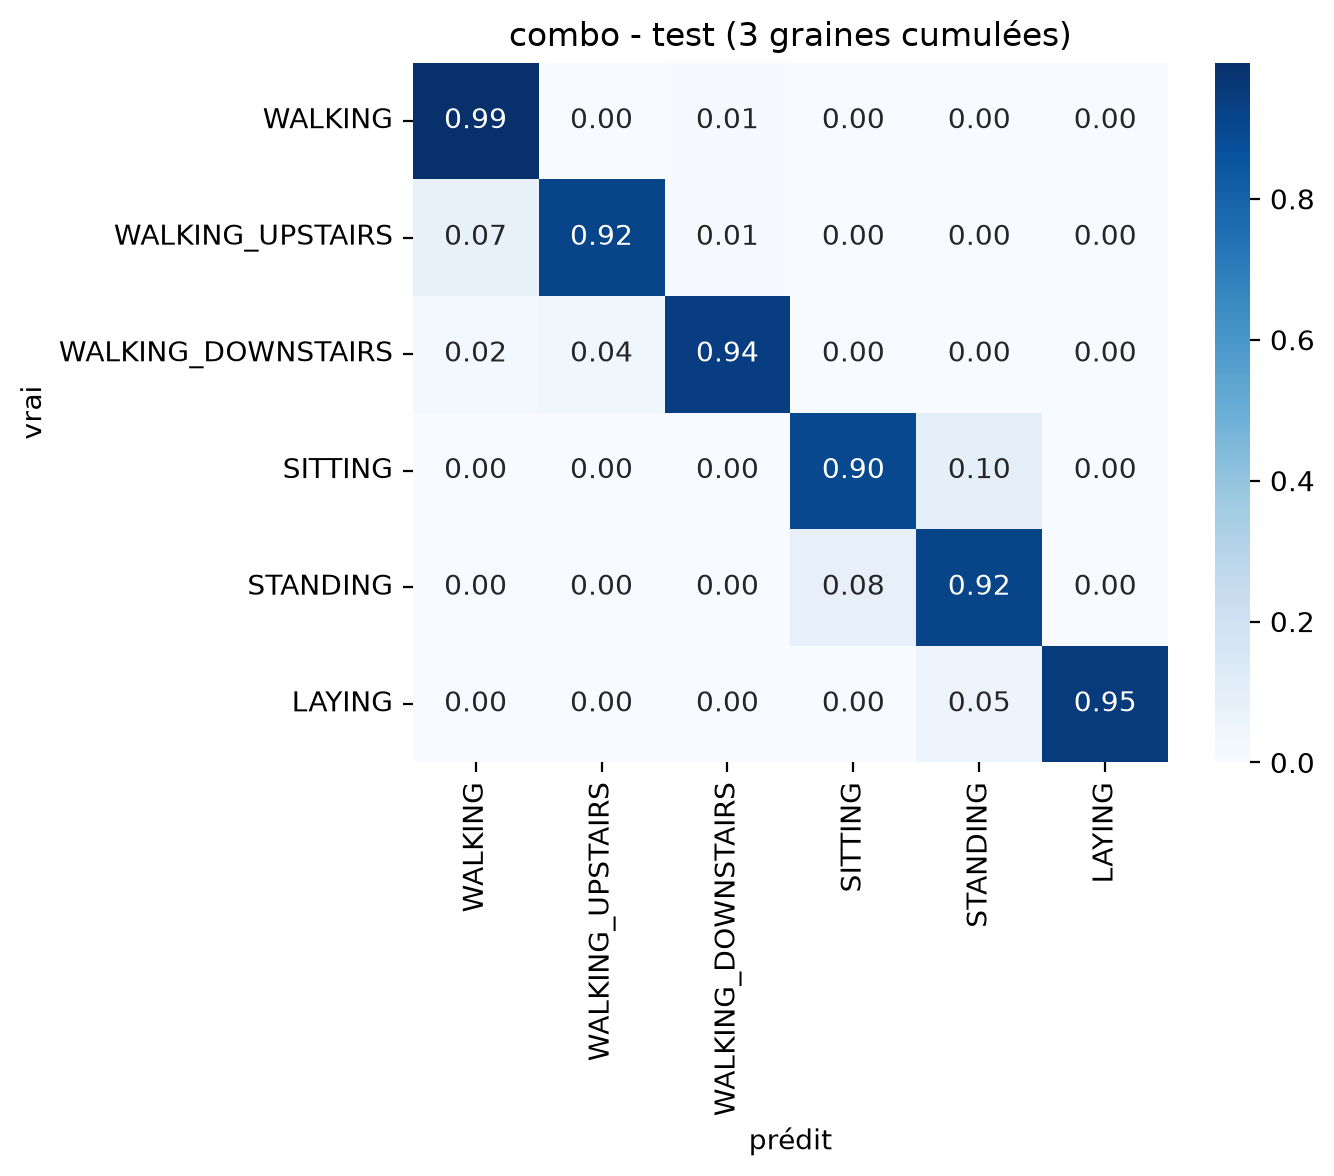
\includegraphics[width=0.32\textwidth]{v2_cm_test_combo}\hfill
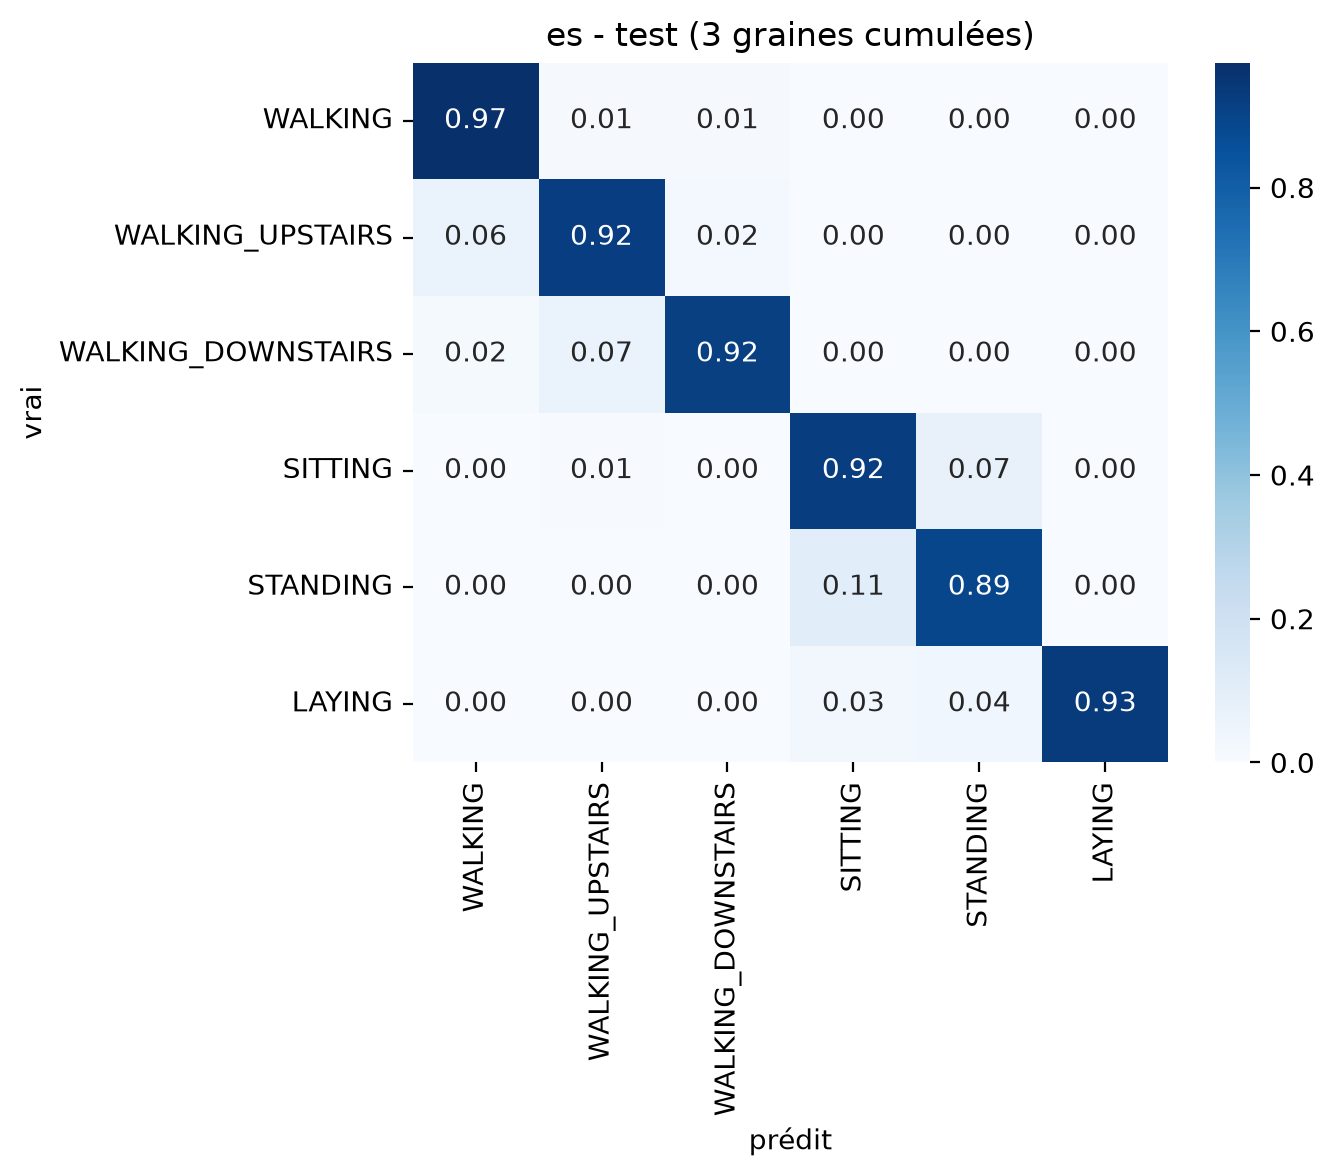
\includegraphics[width=0.32\textwidth]{v2_cm_test_es}\hfill
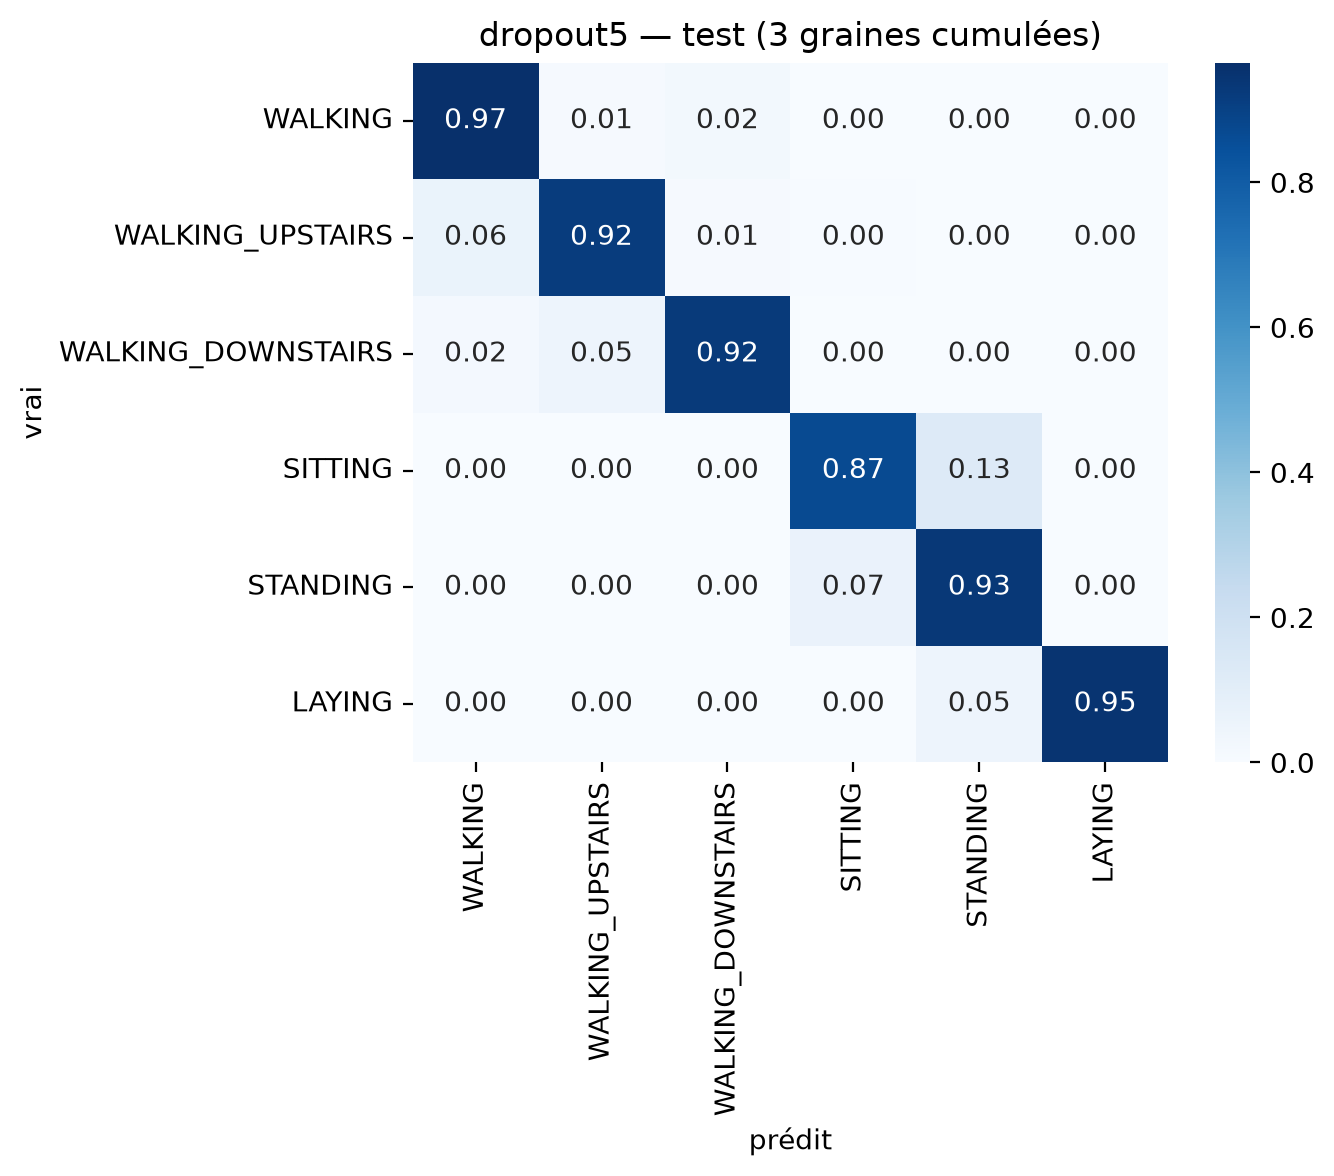
\includegraphics[width=0.32\textwidth]{v2_cm_test_dropout5}
\caption{Matrices de confusion sur le test (3 graines cumulées, normalisées par ligne) :
\texttt{combo}, \texttt{es} et \texttt{dropout5}.}
\label{fig:cm}
\end{figure*}
\subsection{Espace latent : t-SNE et UMAP} % Alioune

\section{Discussion}                  % Madjiguène
\paragraph{Performances.} Hors le réseau à 4 couches sigmoïde qui n'apprend pas, les MLP atteignent un F1 de
0,93 à 0,95, quelle que soit leur taille (36\,k à 187\,k paramètres) : les 561 caractéristiques calculées à la
main sont déjà très informatives, et augmenter la capacité du réseau ne fait qu'accroître le sur-apprentissage.
% Ensemble : gain par rapport à la régression logistique (chiffres d'Alioune).

\paragraph{Généralisation.} Trois niveaux apparaissent : une accuracy d'apprentissage proche de 100\,\%,
environ 94--95\,\% sur les 5 volontaires de validation et 93\,\% sur les 9 volontaires du test, c'est-à-dire sur
des personnes nouvelles. La régularisation (surtout la combinaison avec arrêt anticipé) réduit l'écart
apprentissage--validation de 0,064 à 0,027 et améliore la loss, mais son gain de F1 au test
($+0{,}011$ par rapport à \texttt{es}) reste modeste. Les projections t-SNE et UMAP de la dernière couche cachée
de \texttt{combo} (validation) montrent un recouvrement partiel d'« assis » et « debout » alors que les autres
classes forment des groupes séparés, en accord avec la confusion principale observée au test.

\paragraph{Limites.} La validation ne compte que 5 volontaires, partagés par toutes les comparaisons, et les
écarts-types ne portent que sur la graine d'entraînement : la variabilité due au choix des volontaires (validation
comme test) n'est pas mesurée. Les configurations et l'époque d'arrêt ont été choisies sur cette seule validation,
d'où l'optimisme observé. Avec trois graines, les écarts-types sont peu précis ; nous n'avons pas interprété les
écarts inférieurs à 0,005. Enfin, les explications liées aux capteurs et aux volontaires atypiques restent des
hypothèses.

\section{Conclusion}                  % Ensemble

\section*{Usage d'outils d'IA}       % Ensemble — depuis AI_USAGE.md
Nous avons utilisé l'assistant Claude (Anthropic). Pour la partie de Madjiguène Fall : guidage de la mise en place,
écriture des scripts d'expériences et des cellules du notebook de la version~2, aide à la lecture des tableaux
et à la rédaction des interprétations et de ce rapport. Chaque script a été exécuté, les nombres de paramètres
recalculés, une cellule de contrôle a vérifié que les modèles évalués au test reproduisent les résultats de
validation, et les formulations ont été relues face aux tableaux et figures ; les explications non vérifiées
sont signalées comme hypothèses. Le détail figure dans \texttt{report/AI\_USAGE.md}.
% Alioune : compléter pour sa partie.

\end{document}
